% ============================================================
%  Guía de estudio — Arquitectura de Redes I (PEI 1: Temas 1 y 2)
%  Compilar con:  pdflatex resumen_PEI1_AR1.tex  (dos pasadas)
% ============================================================
\documentclass[11pt,a4paper]{article}

\usepackage[utf8]{inputenc}
\usepackage[T1]{fontenc}
\usepackage{mathpazo}
\usepackage[scaled=.92]{helvet}
\IfFileExists{spanish.ldf}{%
	\usepackage[spanish,es-noshorthands]{babel}\decimalpoint
}{%
	\renewcommand{\contentsname}{Índice}\renewcommand{\tablename}{Tabla}\renewcommand{\figurename}{Figura}%
}
\usepackage[margin=2.2cm,top=2.6cm,bottom=2.4cm]{geometry}
\usepackage[table]{xcolor}
\usepackage{amsmath,amssymb}
\usepackage{booktabs,array,tabularx,longtable}
\usepackage{enumitem}
\usepackage{microtype}
\usepackage{fancyhdr}
\usepackage{titlesec}
\usepackage{tikz}
\usetikzlibrary{arrows.meta,positioning,calc,shapes.geometric}
\usepackage[most]{tcolorbox}
\usepackage{listings}
\usepackage[colorlinks=true,linkcolor=uahblue,urlcolor=uahblue]{hyperref}

% ---------- Colores ----------
\definecolor{uahblue}{RGB}{0,86,164}
\definecolor{uahsand}{RGB}{234,224,200}
\definecolor{okgreen}{RGB}{30,120,70}
\definecolor{warnred}{RGB}{170,40,40}
\definecolor{codebg}{RGB}{248,248,246}
\definecolor{codegray}{RGB}{110,110,110}

% ---------- Títulos ----------
\titleformat{\section}{\Large\sffamily\bfseries\color{uahblue}}{\thesection.}{0.6em}{}[\vspace{-0.5em}\color{uahblue}\titlerule]
\titleformat{\subsection}{\large\sffamily\bfseries\color{uahblue}}{\thesubsection}{0.6em}{}
\titleformat{\subsubsection}{\normalsize\sffamily\bfseries\color{uahblue!80!black}}{}{0em}{}
\titlespacing*{\section}{0pt}{1.6em}{0.9em}
\titlespacing*{\subsection}{0pt}{1.2em}{0.5em}
\titlespacing*{\subsubsection}{0pt}{1em}{0.3em}

% ---------- Cabecera y pie ----------
\pagestyle{fancy}
\fancyhf{}
\renewcommand{\headrule}{\hbox to\headwidth{\color{uahblue}\leaders\hrule height 0.4pt\hfill}}
\lhead{\small\sffamily\color{uahblue}\textbf{Arquitectura de Redes I}}
\rhead{\small\sffamily\color{gray}Guía de estudio PEI\,1 --- Temas 1 y 2}
\cfoot{\small\thepage}
\setlength{\headheight}{22pt}

\setlist{itemsep=2pt,topsep=4pt}
\setlength{\parindent}{0pt}
\setlength{\parskip}{5pt}
\renewcommand{\arraystretch}{1.25}

% ---------- Cajas ----------
\newtcolorbox{definicion}[1][]{colback=uahblue!6,colframe=uahblue,boxrule=0.6pt,arc=2pt,
  left=8pt,right=8pt,top=5pt,bottom=5pt,title={#1},fonttitle=\sffamily\bfseries,breakable}
\newtcolorbox{formula}[1][]{colback=okgreen!6,colframe=okgreen,boxrule=0.6pt,arc=2pt,
  left=8pt,right=8pt,top=5pt,bottom=5pt,title={#1},fonttitle=\sffamily\bfseries,breakable}
\newtcolorbox{ojo}[1][]{colback=warnred!5,colframe=warnred,boxrule=0.6pt,arc=2pt,
  left=8pt,right=8pt,top=5pt,bottom=5pt,title={#1},fonttitle=\sffamily\bfseries,breakable}
\newtcolorbox{nota}[1][]{colback=uahsand!45,colframe=uahsand!90!black,coltitle=black,boxrule=0.6pt,arc=2pt,
  left=8pt,right=8pt,top=5pt,bottom=5pt,title={#1},fonttitle=\sffamily\bfseries,breakable}

\newcolumntype{L}[1]{>{\raggedright\arraybackslash}p{#1}}
\newcommand{\hd}[1]{\cellcolor{uahblue}\textcolor{white}{\textbf{#1}}}
\newcommand{\en}[1]{\emph{(#1)}}

% ---------- Código ----------
\lstset{
  basicstyle=\ttfamily\small,
  backgroundcolor=\color{codebg},
  frame=single,
  rulecolor=\color{uahblue!40},
  keywordstyle=\color{uahblue}\bfseries,
  commentstyle=\color{codegray}\itshape,
  stringstyle=\color{okgreen!70!black},
  showstringspaces=false,
  breaklines=true,
  columns=fixed,basewidth=0.5em,
  keepspaces=true,
  aboveskip=6pt,belowskip=6pt,
  xleftmargin=2pt,xrightmargin=2pt
}
\lstdefinelanguage{pyr}{
  morekeywords={from,import,while,True,input,print,def,with,as,if,else},
  sensitive=true, morecomment=[l]{\#}, morestring=[b]', morestring=[b]"
}
\lstdefinelanguage{httpmsg}{}

\begin{document}

% ============================================================
%  CABECERA DEL DOCUMENTO
% ============================================================
\begin{tcolorbox}[colback=uahblue,colframe=uahblue,arc=0pt,top=14pt,bottom=14pt,left=14pt,right=14pt]
{\sffamily\Huge\bfseries\color{white}Guía de estudio}\\[4pt]
{\sffamily\Large\color{white}Arquitectura de Redes I --- PEI\,1}\\[4pt]
{\sffamily\color{white!85!uahblue}Tema 1: Arquitecturas de red \quad|\quad Tema 2: Protocolos de la capa de aplicación}
\end{tcolorbox}

\begin{definicion}[Qué entra en la PEI\,1 (guía docente 2026/27)]
La PEI\,1 se hace hacia mitad de cuatrimestre, pesa el \textbf{30\,\%} y cubre los \textbf{Temas 1 y 2}, con teoría y problemas (cuestiones de desarrollo o test y ejercicios). Resultados de aprendizaje evaluados: RA1--RA8, RA10 y RA11.
\vspace{2pt}
\begin{tabularx}{\linewidth}{@{}L{6.4cm}X@{}}
\toprule
\hd{Contenido oficial} & \hd{Dónde está en esta guía} \\
\midrule
T1: elementos de red, protocolos, retardos, lógica de redes, OSI, TCP/IP & Sección 1 (RA1--RA6) \\
T2: aplicaciones distribuidas, cliente/servidor, HTTP, DNS, sockets & Sección 2 (RA7, RA8, RA10) \\
Cálculo de parámetros de eficiencia & Subsecciones 1.2 y 1.4, ejercicios y hoja de fórmulas (RA6) \\
\bottomrule
\end{tabularx}

El SMTP/correo no figura en los contenidos oficiales (solo web y DNS), por eso no se desarrolla.
\end{definicion}

\begin{definicion}[Cómo usar esta guía]
Resumen de los \textbf{Temas 1 y 2} (PEI\,1, 30\,\% de la nota) basado en el resumen previo, revisado y ampliado con \emph{Redes de computadoras: un enfoque descendente} (Kurose \& Ross, 7.\textsuperscript{a} ed.).
\begin{itemize}[leftmargin=1.2em]
  \item Las cajas \textbf{verdes} contienen fórmulas.
  \item Las cajas \textbf{rojas} marcan errores frecuentes de examen.
  \item Al final hay \textbf{ejercicios resueltos} y una \textbf{hoja de fórmulas}.
  \item La última sección lista las \textbf{correcciones} hechas respecto al resumen original.
\end{itemize}
\end{definicion}

\tableofcontents
\newpage

% ============================================================
%  TEMA 1
% ============================================================
\section{Tema 1: Arquitecturas de red}

% ------------------------------------------------------------
\subsection{Elementos de una red}

Internet es una red de redes formada por miles de millones de dispositivos, \emph{enlaces} y \emph{conmutadores de paquetes}. Se describe en tres partes:

\begin{itemize}
  \item \textbf{Borde de la red.} Sistemas finales (\emph{hosts}) que ejecutan aplicaciones. Se agrupan en \textbf{clientes} (PC, móviles, dispositivos IoT, que inician peticiones) y \textbf{servidores} (máquinas en centros de datos que atienden peticiones y distribuyen contenido).
  \item \textbf{Redes de acceso.} Enlaces que conectan un sistema final con el primer router (\emph{edge router}).
  \item \textbf{Núcleo de la red.} Malla de routers interconectados con enlaces de alta capacidad (fibra óptica terrestre y submarina) que transporta los datos de la red de acceso de origen a la de destino.
\end{itemize}

\subsubsection{Tecnologías de acceso}

\begin{tabularx}{\textwidth}{@{}L{2.6cm}L{3.3cm}X@{}}
\toprule
\hd{Tecnología} & \hd{Medio} & \hd{Características clave} \\
\midrule
\textbf{FTTH} \en{fibra hasta el hogar} & Fibra óptica & Fibra hasta la vivienda. Arquitectura típica PON (óptica pasiva): un divisor óptico reparte la fibra entre varios hogares. GPON es asimétrica (en torno a 2{,}5 Gbps de bajada y 1{,}25 Gbps de subida); XGS-PON ofrece 10 Gbps simétricos. \\
\textbf{HFC} \en{híbrido fibra-coaxial} & Fibra hasta el nodo de zona y coaxial hasta el hogar & Medio \textbf{compartido} entre los usuarios del vecindario. Usa el estándar \textbf{DOCSIS}. Canales de bajada y subida \textbf{asimétricos}. \\
\textbf{DSL} & Par trenzado de cobre de la red telefónica & Línea \textbf{dedicada} hasta la central. Con \textbf{FDM} se divide en tres bandas: telefonía bidireccional (hasta 4~kHz), subida (4--50~kHz) y bajada (50~kHz--1~MHz). La velocidad cae con la distancia a la central. \\
\textbf{Ethernet} (IEEE 802.3) & Par trenzado (UTP Cat\,5e/6/7) con conectores RJ-45; también fibra & Acceso LAN en empresas, universidades y hogares mediante \emph{switches}. Velocidades de 100~Mbps, 1~Gbps, 10~Gbps o más. \\
\textbf{Wi-Fi} (IEEE 802.11) & Radio, bandas sin licencia (2{,}4, 5 y 6~GHz) & Acceso inalámbrico local mediante un punto de acceso. Usa acceso múltiple (CSMA/CA) para compartir el canal. \\
\textbf{Celular} (4G LTE, 5G NR) & Radio, espectro con licencia & Acceso inalámbrico de área extensa mediante estaciones base (eNodeB / gNodeB), con soporte de movilidad. \\
\bottomrule
\end{tabularx}

\subsubsection{Medios físicos}

\begin{tabularx}{\textwidth}{@{}L{3.2cm}X@{}}
\toprule
\hd{Medio} & \hd{Observaciones} \\
\midrule
Par trenzado & Barato y muy extendido. Velocidades de 100~Mbps a 10~Gbps según categoría y longitud. \\
Cable coaxial & Dos conductores concéntricos. Admite medio compartido y velocidades altas; base de HFC. \\
Fibra óptica & Pulsos de luz. Muy alta velocidad (decenas o cientos de Gbps), baja atenuación e inmunidad al ruido electromagnético. Es el medio del núcleo. \\
Radio terrestre & Sin cableado físico; sensible a interferencias, obstáculos y multitrayecto. \\
Satélite & Geoestacionario (a unos 36\,000~km, con retardo de propagación en torno a 280~ms) o de órbita baja, con retardo mucho menor. \\
\bottomrule
\end{tabularx}

\subsubsection{Clasificación de las redes}

\begin{tabularx}{\textwidth}{@{}L{3.6cm}X@{}}
\toprule
\hd{Criterio} & \hd{Categorías} \\
\midrule
Topología & \textbf{Malla} (cada nodo conectado con varios otros; muy robusta y costosa), \textbf{estrella} (todos los nodos a un nodo central; un fallo central deja la red incomunicada), \textbf{árbol} (jerarquía de estrellas). \\
Alcance geográfico & \textbf{LAN} (edificio o campus), \textbf{MAN} (ciudad o área metropolitana), \textbf{WAN} (país o continente). \\
Cercanía al usuario & \textbf{Acceso} (hasta el usuario), \textbf{agregación} (concentra el tráfico de muchos accesos), \textbf{núcleo} (transporte troncal). \\
Medio con el usuario & \textbf{Cableada} (cobre, fibra) o \textbf{radio} (Wi-Fi, celular, satélite). \\
Movilidad & \textbf{Fija} o \textbf{móvil}. \\
Tipo de servicio & Datos, voz, vídeo, servicios interactivos y multimedia. \\
\bottomrule
\end{tabularx}

% ------------------------------------------------------------
\subsection{Conmutación en el núcleo: circuitos frente a paquetes}

\begin{tabularx}{\textwidth}{@{}L{3.2cm}XX@{}}
\toprule
\hd{Parámetro} & \hd{Conmutación de circuitos} & \hd{Conmutación de paquetes} \\
\midrule
Recursos & Reservados extremo a extremo antes de transmitir. & Sin reserva; compartidos bajo demanda. \\
Garantías & Caudal y retardo garantizados. & Sin garantías (\emph{best effort}); retardo y pérdidas variables. \\
Multiplexación & \textbf{FDM} o \textbf{TDM} con recursos dedicados a cada llamada. & \textbf{Multiplexación estadística}: los paquetes se intercalan según la demanda. \\
Ráfagas & Ineficiente: el circuito reservado se desperdicia en los silencios. & Eficiente: aprovecha la inactividad de otros usuarios. \\
Estado & Establecimiento y cierre de llamada; los conmutadores guardan estado. & Los routers no guardan estado de conexión. \\
Ejemplo & Red telefónica clásica. & Internet. \\
\bottomrule
\end{tabularx}

\subsubsection{Multiplexación en circuitos}

\begin{itemize}
  \item \textbf{FDM} \en{frequency-division multiplexing}: el espectro del enlace se divide en bandas fijas; cada conexión usa su banda en exclusiva durante toda la sesión.
  \item \textbf{TDM} \en{time-division multiplexing}: el tiempo se divide en tramas de duración fija, y cada trama en un número fijo de \emph{ranuras}. Cada conexión dispone de una ranura periódica en cada trama.
\end{itemize}

\subsubsection{Almacenamiento y reenvío}

\begin{definicion}[Store-and-forward]
Un conmutador de paquetes debe recibir el paquete \textbf{completo} (los $L$ bits) antes de empezar a transmitir su primer bit por el enlace de salida. Transmitir $L$ bits a velocidad $R$ tarda $L/R$ segundos.
\end{definicion}

\begin{formula}[Retardo de un paquete a través de $N$ enlaces (sin colas, procesamiento ni propagación)]
\[
d_{\text{extremo-extremo}} = N\,\frac{L}{R}
\]
(con $N-1$ routers intermedios, todos los enlaces a velocidad $R$).
\end{formula}

\subsubsection{Ventaja de la multiplexación estadística}

Ejemplo clásico: un enlace de $1$~Mbps lo comparten usuarios que, cuando están activos, transmiten a $100$~kbps, y que están activos solo el $10$\,\% del tiempo.

\begin{itemize}
  \item Con \textbf{conmutación de circuitos} caben $1\,\text{Mbps}/100\,\text{kbps} = 10$ usuarios, estén activos o no.
  \item Con \textbf{conmutación de paquetes}, con $35$ usuarios, la probabilidad de que más de $10$ estén activos a la vez es $P(N>10)\approx 0{,}0004$ (distribución binomial). Casi nunca hay congestión, y se sirve a $3{,}5$ veces más usuarios.
\end{itemize}

\begin{ojo}[Error frecuente]
La conmutación de paquetes \emph{no} es siempre mejor. Para tráfico constante y con exigencias de tiempo real, la reserva de circuitos tiene sentido. Compara siempre tráfico en ráfagas frente a tráfico continuo.
\end{ojo}

% ------------------------------------------------------------
\subsection{Estructura de Internet y normalización}

\subsubsection{Estructura de Internet}
\begin{itemize}
  \item Los usuarios se conectan a \textbf{ISP de acceso}. Los ISP se interconectan entre sí, de forma que dos hosts cualesquiera pueden comunicarse.
  \item Los ISP de nivel superior (\emph{tier-1}) forman la espina dorsal. Los ISP se interconectan directamente (\emph{peering}) o mediante \textbf{puntos neutros de intercambio} (IXP).
  \item Grandes proveedores de contenido operan sus propias redes y centros de datos, acercando el contenido a los usuarios.
\end{itemize}

\subsubsection{Organismos de normalización}

\begin{tabularx}{\textwidth}{@{}L{3.2cm}X@{}}
\toprule
\hd{Organismo} & \hd{Papel} \\
\midrule
\textbf{IETF} & Desarrolla los estándares de Internet, publicados como documentos \textbf{RFC} (\emph{Request For Comments}): TCP, IP, HTTP, SMTP, DNS, etc. \\
\textbf{IEEE 802} & Estándares de redes locales y metropolitanas: Ethernet (802.3) y Wi-Fi (802.11). \\
\textbf{ITU} & Estándares de telecomunicaciones (organismo de Naciones Unidas). \\
\textbf{ISO} & Estándares generales; autora del modelo de referencia OSI. \\
\textbf{W3C} & Estándares de la web (HTML, CSS, etc.). \\
\textbf{ICANN / IANA} & Gestión de direcciones IP, nombres de dominio y números de puerto asignados. \\
\bottomrule
\end{tabularx}

La \textbf{regulación} (licencias de espectro, competencia entre operadores, obligaciones de servicio) la ejercen organismos públicos nacionales e internacionales; en España, por ejemplo, el ministerio competente en telecomunicaciones y la CNMC. Normalizar sirve para la \emph{interoperabilidad}; regular, para ordenar el mercado y el uso de recursos escasos como el espectro.

% ------------------------------------------------------------
\subsection{Retardos, pérdidas y tasa de transferencia}

\subsubsection{Retardo nodal}

\begin{center}
\begin{tikzpicture}[font=\small\sffamily,
  blk/.style={draw=uahblue,fill=uahblue!8,rounded corners=2pt,minimum height=1.0cm,minimum width=2.5cm,align=center},
  arr/.style={-{Stealth[length=2.5mm]},thick,uahblue}]
  \node[blk] (a) {$d_{\text{proc}}$\\[-1pt]\scriptsize leer cabecera};
  \node[blk,right=0.7cm of a] (b) {$d_{\text{cola}}$\\[-1pt]\scriptsize espera en búfer};
  \node[blk,right=0.7cm of b] (c) {$d_{\text{trans}}$\\[-1pt]\scriptsize volcar los bits};
  \node[blk,right=0.7cm of c,fill=uahsand!60] (d) {$d_{\text{prop}}$\\[-1pt]\scriptsize viaje por el enlace};
  \draw[arr] (a)--(b); \draw[arr] (b)--(c); \draw[arr] (c)--(d);
  \node[above=2pt of a,anchor=south west,xshift=-6pt] {Paquete entrante};
\end{tikzpicture}
\end{center}

\begin{formula}[Retardo nodal]
\[
d_{\text{nodal}} = d_{\text{proc}} + d_{\text{cola}} + d_{\text{trans}} + d_{\text{prop}}
\]
\end{formula}

\begin{tabularx}{\textwidth}{@{}L{3cm}X@{}}
\toprule
\hd{Componente} & \hd{Descripción} \\
\midrule
$d_{\text{proc}}$ & Examinar la cabecera, comprobar errores y decidir la interfaz de salida con la tabla de reenvío. Del orden de microsegundos o menos. \\
$d_{\text{cola}}$ & Espera en la cola de salida hasta empezar a transmitirse. \textbf{Variable}: depende del tráfico. \\
$d_{\text{trans}}=L/R$ & Tiempo de volcar los $L$ bits al enlace a $R$ bps. Depende del \textbf{tamaño} y de la \textbf{velocidad} del enlace, no de la distancia. \\
$d_{\text{prop}}=d/s$ & Tiempo que tarda un bit en recorrer el enlace de longitud $d$ a velocidad de propagación $s$ ($\approx 2\cdot10^{8}$~m/s en fibra y cobre, hasta $3\cdot10^{8}$~m/s en el vacío). Depende de la \textbf{distancia}, no del tamaño del paquete. \\
\bottomrule
\end{tabularx}

\begin{ojo}[No confundir $d_{\text{trans}}$ con $d_{\text{prop}}$]
$d_{\text{trans}}$ es el tiempo de \emph{meter} el paquete en el enlace (depende de $L$ y $R$). $d_{\text{prop}}$ es el tiempo de \emph{recorrer} el enlace (depende de $d$ y $s$). Analogía: una caravana de coches que pasa por un peaje (transmisión) y luego viaja por la carretera (propagación).
\end{ojo}

\subsubsection{Retardo de cola e intensidad de tráfico}

\begin{formula}[Intensidad de tráfico]
\[
\text{Intensidad de tráfico}=\frac{L\cdot a}{R}
\]
$L$: tamaño medio del paquete (bits); $a$: tasa media de llegada (paquetes/s); $R$: velocidad de transmisión (bps).
\end{formula}

\begin{itemize}
  \item Si $La/R \approx 0$: el retardo de cola medio es prácticamente nulo.
  \item Si $La/R \to 1$: el retardo medio de cola \textbf{crece rápidamente} (sin límite en una cola infinita).
  \item Si $La/R > 1$: llega más tráfico del que el enlace puede sacar. La cola crece sin parar o, si es finita, \textbf{se desborda} y se pierden paquetes.
\end{itemize}

\textbf{Pérdida de paquetes.} Las colas reales son finitas: si un paquete llega a una cola llena, el router lo descarta. El porcentaje de pérdidas crece con la intensidad de tráfico. Un paquete perdido puede retransmitirse extremo a extremo (lo hará TCP, Tema 3).

\subsubsection{Retardo extremo a extremo}

\begin{formula}[$N$ enlaces idénticos, sin colas]
\[
d_{\text{extremo-extremo}} = N\,\bigl(d_{\text{proc}} + d_{\text{trans}} + d_{\text{prop}}\bigr)
\]
Se cuentan $N$ transmisiones: la del host origen más las de los $N-1$ routers.
\end{formula}

\subsubsection{Tasa de transferencia (\emph{throughput})}

\begin{itemize}
  \item \textbf{Instantánea}: velocidad a la que el receptor recibe el archivo en un instante dado.
  \item \textbf{Media}: $F/T$ bps para un archivo de $F$ bits recibido en $T$ segundos.
  \item En un camino con enlaces de velocidades $R_1,\dots,R_N$ el cuello de botella limita:
\end{itemize}

\begin{formula}[Throughput extremo a extremo]
\[
\text{throughput}=\min\{R_1,R_2,\dots,R_N\},\qquad T=\frac{F}{\text{throughput}}
\]
\end{formula}

\subsubsection{Producto ancho de banda-retardo}

\begin{nota}[Dos definiciones, según el contexto]
\begin{itemize}
  \item En Kurose \& Ross (cap.~1) el producto ancho de banda-retardo es $R\cdot d_{\text{prop}}$: el \textbf{máximo número de bits que caben en el enlace} a la vez.
  \item En el contexto de transporte (Tema 3) se usa $R\cdot \text{RTT}$: los bits \emph{en vuelo} que el emisor puede enviar antes de recibir el primer reconocimiento. Determina el tamaño de ventana necesario para llenar la tubería.
\end{itemize}
Lee el enunciado para ver cuál se pide; en problemas del Tema 1 suele ser $R\cdot d_{\text{prop}}$.
\end{nota}

% ------------------------------------------------------------
\subsection{Protocolos y arquitectura en capas}

\begin{definicion}[Protocolo]
Un protocolo define el \textbf{formato} y el \textbf{orden} de los mensajes intercambiados entre entidades pares, y las \textbf{acciones} que deben ejecutarse al enviar o recibir un mensaje o al ocurrir un evento (por ejemplo, un temporizador que vence).
\end{definicion}

La arquitectura en capas divide un problema complejo en partes. Cada capa ofrece un \textbf{servicio} a la capa superior apoyándose en los servicios de la inferior, y oculta los detalles de su implementación. Ventajas: modularidad y facilidad de mantenimiento; inconveniente: posible duplicación de funciones y sobrecarga de cabeceras.

\subsubsection{Modelo OSI y pila TCP/IP}

\begin{center}
\begin{tikzpicture}[font=\small\sffamily,
  l/.style={draw=uahblue,fill=uahblue!8,minimum width=4.2cm,minimum height=0.7cm,align=center},
  m/.style={draw=uahblue,fill=uahsand!60,minimum width=4.6cm,align=center},
  arr/.style={-{Stealth[length=2.2mm]},uahblue}]
  \node[font=\sffamily\bfseries\color{uahblue}] at (0,6.0) {Modelo OSI (7 capas)};
  \node[font=\sffamily\bfseries\color{uahblue}] at (7.4,6.0) {Pila TCP/IP (5 capas)};
  \node[l] at (0,0.0) {1. Física};
  \node[l] at (0,0.8) {2. Enlace de datos};
  \node[l] at (0,1.6) {3. Red};
  \node[l] at (0,2.4) {4. Transporte};
  \node[l] at (0,3.2) {5. Sesión};
  \node[l] at (0,4.0) {6. Presentación};
  \node[l] at (0,4.8) {7. Aplicación};
  \node[m] at (7.4,0.0) {1. Física};
  \node[m] at (7.4,0.8) {2. Enlace\\[-2pt]\scriptsize Ethernet, Wi-Fi};
  \node[m,minimum height=0.7cm] at (7.4,1.6) {3. Red\\[-2pt]\scriptsize IP, ICMP, enrutamiento};
  \node[m] at (7.4,2.4) {4. Transporte\\[-2pt]\scriptsize TCP, UDP};
  \node[m,minimum height=2.3cm] at (7.4,4.0) {5. Aplicación\\[-2pt]\scriptsize HTTP, DNS, SMTP, FTP, SSH};
  \foreach \y in {0,0.8,1.6,2.4}{\draw[arr] (2.15,\y)--(5.05,\y);}
  \draw[arr] (2.15,4.0)--(5.05,4.0);
\end{tikzpicture}
\end{center}

\begin{tabularx}{\textwidth}{@{}L{2.8cm}L{3.2cm}X@{}}
\toprule
\hd{Capa} & \hd{PDU} & \hd{Función} \\
\midrule
Aplicación & Mensaje & Soporta las aplicaciones de red; define el formato de los mensajes de protocolos como HTTP, DNS o SMTP. \\
Transporte & Segmento & Transferencia lógica \textbf{proceso a proceso}; multiplexa aplicaciones con números de puerto. TCP es fiable y UDP no. \\
Red & Datagrama IP & Entrega \textbf{host a host} a través de varias redes: direccionamiento IP y enrutamiento. \\
Enlace & Trama (\emph{frame}) & Transfiere tramas entre nodos \textbf{adyacentes}; direccionamiento MAC, acceso al medio y detección de errores. \\
Física & Bit & Transmite bits individuales por el medio (voltajes, frecuencias, tiempos de bit). \\
\bottomrule
\end{tabularx}

\begin{nota}[Capas de OSI que TCP/IP no distingue]
En OSI, \emph{presentación} (cifrado, compresión, formato de datos) y \emph{sesión} (sincronización, recuperación) son capas propias. En TCP/IP, si hacen falta, las implementa la aplicación.
\end{nota}

\begin{nota}[Terminología del PDU de UDP]
En Kurose \& Ross, la PDU de transporte se llama \emph{segmento} tanto en TCP como en UDP. Muchos textos llaman \emph{datagrama} al paquete UDP. Ambos usos son habituales: usa el término que emplee tu profesor y ten presentes los dos.
\end{nota}

\subsubsection{Encapsulamiento}

Cada capa añade su \textbf{cabecera} (y la de enlace, también una cola o \emph{trailer}) al descender por la pila; en el receptor se retiran en orden inverso.

\begin{center}
\begin{tikzpicture}[font=\small\sffamily,
  ht/.style={draw=black!60,fill=uahblue!25,minimum height=0.65cm,minimum width=1.2cm,inner sep=2pt},
  dt/.style={draw=black!60,fill=uahsand!70,minimum height=0.65cm,minimum width=3.6cm,inner sep=2pt}]
  % Aplicación
  \node[dt,anchor=west] at (3.6,3.0) (m1) {Mensaje};
  \node[anchor=east,font=\sffamily\small\bfseries] at (-0.2,3.0) {Aplicación};
  % Transporte
  \node[ht,anchor=west] at (2.4,2.1) (a2) {$H_t$};
  \node[dt,anchor=west] at (3.6,2.1) {Mensaje};
  \node[anchor=east,font=\sffamily\small\bfseries] at (-0.2,2.1) {Transporte};
  \node[anchor=west,font=\small] at (8.4,2.1) {Segmento};
  % Red
  \node[ht,anchor=west] at (1.2,1.2) {$H_r$};
  \node[ht,anchor=west] at (2.4,1.2) {$H_t$};
  \node[dt,anchor=west] at (3.6,1.2) {Mensaje};
  \node[anchor=east,font=\sffamily\small\bfseries] at (-0.2,1.2) {Red};
  \node[anchor=west,font=\small] at (8.4,1.2) {Datagrama};
  % Enlace
  \node[ht,anchor=west] at (0.0,0.3) {$H_e$};
  \node[ht,anchor=west] at (1.2,0.3) {$H_r$};
  \node[ht,anchor=west] at (2.4,0.3) {$H_t$};
  \node[dt,anchor=west] at (3.6,0.3) {Mensaje};
  \node[ht,anchor=west,fill=black!10] at (7.2,0.3) {$T_e$};
  \node[anchor=east,font=\sffamily\small\bfseries] at (-0.2,0.3) {Enlace};
  \node[anchor=west,font=\small] at (8.4,0.3) {Trama};
\end{tikzpicture}
\end{center}

\textbf{Dispositivos y capas.} Un \emph{host} implementa las cinco capas. Un \emph{router} implementa física, enlace y red. Un \emph{switch} de enlace implementa física y enlace.

% ============================================================
%  TEMA 2
% ============================================================
\newpage
\section{Tema 2: Protocolos de la capa de aplicación}

% ------------------------------------------------------------
\subsection{Principios de las aplicaciones de red}

Una aplicación de red está formada por programas que se ejecutan en distintos sistemas finales y se comunican a través de la red. No se programa código para los routers del núcleo.

\begin{center}
\begin{tikzpicture}[font=\small\sffamily,
  n/.style={draw=uahblue,fill=uahblue!8,rounded corners=2pt,minimum width=1.7cm,minimum height=0.8cm,align=center},
  s/.style={draw=uahblue,fill=uahsand!60,rounded corners=2pt,minimum width=2.2cm,minimum height=0.9cm,align=center},
  a/.style={-{Stealth[length=2.2mm]},uahblue},
  t/.style={font=\sffamily\bfseries\color{uahblue}}]
  \node[t] at (1.8,2.6) {Cliente-servidor};
  \node[s] (srv) at (1.8,1.4) {Servidor\\[-2pt]\scriptsize IP fija};
  \node[n] (c1) at (0,-0.4) {Cliente};
  \node[n] (c2) at (3.6,-0.4) {Cliente};
  \draw[a,<->] (c1)--(srv); \draw[a,<->] (c2)--(srv);
  \node[t] at (9,2.6) {Peer-to-peer (P2P)};
  \node[n] (p1) at (8,1.4) {Par A};
  \node[n] (p2) at (10,1.4) {Par B};
  \node[n] (p3) at (9,-0.4) {Par C};
  \draw[a,<->] (p1)--(p2); \draw[a,<->] (p1)--(p3); \draw[a,<->] (p2)--(p3);
\end{tikzpicture}
\end{center}

\begin{tabularx}{\textwidth}{@{}L{2.8cm}XX@{}}
\toprule
 & \hd{Cliente-servidor} & \hd{P2P} \\
\midrule
Servidor & Siempre activo, con \textbf{IP fija} y conocida; suele ser una granja de servidores. & Sin servidor dedicado permanente. \\
Clientes / pares & Se conectan de forma intermitente, con IP posiblemente dinámica; \textbf{no se comunican entre sí}. & Se conectan de forma intermitente, cambian de IP y \textbf{se comunican directamente}. \\
Escalabilidad & Limitada por el servidor y su ancho de banda. & \textbf{Autoescalable}: cada par que entra aporta capacidad (descarga y subida). \\
Dificultad & Sencilla de gestionar. & Gestión compleja: seguridad, incentivos, conectividad. \\
\bottomrule
\end{tabularx}

\begin{formula}[Tiempo de distribución de un archivo de $F$ bits a $N$ pares]
$u_s$: subida del servidor; $u_i$: subida del par $i$; $d_{\min}$: menor bajada entre los pares.
\[
D_{\text{CS}}\ \ge\ \max\Bigl\{\frac{N F}{u_s},\ \frac{F}{d_{\min}}\Bigr\},\qquad
D_{\text{P2P}}\ \ge\ \max\Bigl\{\frac{F}{u_s},\ \frac{F}{d_{\min}},\ \frac{N F}{u_s+\sum_{i=1}^{N}u_i}\Bigr\}
\]
En cliente-servidor el tiempo crece \emph{linealmente} con $N$; en P2P la capacidad de subida total crece con $N$, y el tiempo tiende a un valor acotado.
\end{formula}

\subsubsection{Procesos, sockets y direccionamiento}
\begin{itemize}
  \item Se comunican \textbf{procesos}, no máquinas. El que inicia la comunicación es el \textbf{cliente}; el que espera, el \textbf{servidor}.
  \item El \textbf{socket} es la interfaz (API) entre el proceso de aplicación y la capa de transporte del sistema operativo.
  \item Para identificar un proceso destino se necesitan dos datos: la \textbf{dirección IP} del host (32 bits en IPv4, 128 en IPv6) y el \textbf{número de puerto} (16 bits, $0$--$65\,535$).
  \item \emph{Puertos bien conocidos} ($0$--$1023$), asignados por IANA: HTTP 80, HTTPS 443, DNS 53, SSH 22, SMTP 25.
\end{itemize}

\subsubsection{Qué necesita una aplicación del transporte}

\begin{tabularx}{\textwidth}{@{}L{3.6cm}X@{}}
\toprule
\hd{Requisito} & \hd{Ejemplo} \\
\midrule
Transferencia fiable de datos & Imprescindible en correo, transferencia de archivos y web; tolerable cierta pérdida en audio y vídeo en tiempo real. \\
Tasa de transferencia & Aplicaciones \emph{sensibles al ancho de banda} (vídeo) frente a \emph{elásticas} (correo, web). \\
Temporización & Telefonía y juegos en red exigen retardos bajos. \\
Seguridad & Confidencialidad, integridad, autenticación (cifrado con TLS). \\
\bottomrule
\end{tabularx}

% ------------------------------------------------------------
\subsection{Servicios de transporte: TCP frente a UDP}

\begin{tabularx}{\textwidth}{@{}L{3.6cm}XX@{}}
\toprule
 & \hd{TCP} & \hd{UDP} \\
\midrule
Conexión & Orientado a conexión: \emph{handshake} de tres vías antes de enviar datos. & Sin conexión: se envía directamente. \\
Fiabilidad & Sin pérdidas, sin duplicados, en orden. & No fiable: sin garantías de entrega ni de orden. \\
Control de flujo & Sí (ventana de recepción). & No. \\
Control de congestión & Sí. & No. \\
Cabecera & 20 bytes como mínimo. & \textbf{8 bytes}. \\
Garantías de tasa o retardo & \textbf{Ninguna}. & \textbf{Ninguna}. \\
Usos típicos & Web, correo, archivos, SSH. & DNS, VoIP, streaming, juegos en red. \\
\bottomrule
\end{tabularx}

\textbf{Cabecera UDP} (cuatro campos de 16 bits):

\begin{center}
\begin{tabular}{|c|c|}
\hline
\textbf{Puerto origen} & \textbf{Puerto destino} \\ \hline
\textbf{Longitud} & \textbf{Suma de comprobación} \\ \hline
\multicolumn{2}{|c|}{Datos de aplicación} \\ \hline
\end{tabular}
\end{center}

\textbf{TCP en una frase.} Garantiza que los bytes llegan sin errores, sin huecos, sin duplicados y en orden, mediante números de secuencia, reconocimientos acumulativos (ACK) y temporizador de retransmisión (RTO); el control de flujo evita saturar el receptor (ventana de recepción \texttt{rwnd}) y el control de congestión protege la red (ventana de congestión \texttt{cwnd}). Se estudia en detalle en el Tema 3.

\begin{ojo}[Error frecuente]
TCP \emph{no} garantiza ancho de banda mínimo ni retardo máximo. Ofrece fiabilidad, no rendimiento garantizado. Y los servicios de seguridad (TLS) no forman parte de TCP: se añaden en la capa de aplicación.
\end{ojo}

\begin{tabularx}{\textwidth}{@{}L{3.6cm}L{4.0cm}L{3cm}@{}}
\toprule
\hd{Aplicación} & \hd{Protocolo de aplicación} & \hd{Transporte} \\
\midrule
Web & HTTP, HTTPS & TCP \\
Correo electrónico & SMTP & TCP \\
Resolución de nombres & DNS & UDP (TCP para transferencias de zona) \\
Transferencia de archivos & FTP & TCP \\
Acceso remoto & SSH & TCP \\
Telefonía por Internet & Propietario (p.\,ej., RTP) & Normalmente UDP \\
\bottomrule
\end{tabularx}

% ------------------------------------------------------------
\subsection{La web y HTTP}

\begin{definicion}[HTTP \en{HyperText Transfer Protocol}]
Protocolo de aplicación de la web, con el modelo cliente-servidor: el navegador pide objetos (HTML, imágenes, scripts\dots) y el servidor web los devuelve. Cada objeto se identifica con una URL. Usa \textbf{TCP}, puerto 80 (443 en HTTPS). Es un protocolo \textbf{sin estado}: el servidor no guarda información de peticiones anteriores del cliente.
\end{definicion}

\subsubsection{Formato de los mensajes}

Los mensajes son texto ASCII legible. \textbf{Petición}:

\begin{lstlisting}[language=httpmsg]
GET /index.html HTTP/1.1          <- linea de peticion
Host: www.uah.es                  <- cabeceras
Connection: close
User-Agent: Mozilla/5.0
Accept-Language: es
                                  <- linea en blanco (fin de cabeceras)
\end{lstlisting}

\textbf{Respuesta}:

\begin{lstlisting}[language=httpmsg]
HTTP/1.1 200 OK                   <- linea de estado
Connection: close
Date: Sat, 07 Nov 2026 10:00:00 GMT
Server: Apache
Last-Modified: Fri, 06 Nov 2026 09:00:00 GMT
Content-Length: 6821
Content-Type: text/html
                                  <- linea en blanco
(datos: el objeto solicitado)     <- cuerpo
\end{lstlisting}

\subsubsection{Métodos}

\begin{tabularx}{\textwidth}{@{}L{2.2cm}X@{}}
\toprule
\hd{Método} & \hd{Uso} \\
\midrule
\texttt{GET} & Pide el objeto identificado por la URL. Los parámetros pueden ir en la propia URL. \\
\texttt{POST} & Envía datos (por ejemplo, un formulario) en el cuerpo del mensaje. \\
\texttt{HEAD} & Como GET, pero el servidor omite el cuerpo; útil para depuración. \\
\texttt{PUT} & Sube un objeto al servidor, reemplazando el recurso de la URL. \\
\texttt{DELETE} & Borra el objeto de la URL en el servidor. \\
\bottomrule
\end{tabularx}

\subsubsection{Códigos de estado}

\begin{tabularx}{\textwidth}{@{}L{1.4cm}L{4.4cm}X@{}}
\toprule
\hd{Código} & \hd{Nombre} & \hd{Significado} \\
\midrule
\textbf{200} & OK & Petición correcta; el objeto va en la respuesta. \\
\textbf{301} & Moved Permanently & Recurso movido de forma definitiva; la nueva URL va en la cabecera \texttt{Location}. \\
\textbf{304} & Not Modified & La copia en caché del cliente está al día; no se envía el cuerpo. \\
\textbf{400} & Bad Request & Petición malformada. \\
\textbf{404} & Not Found & El recurso no existe en el servidor. \\
\textbf{418} & I'm a teapot & El servidor se niega a preparar café porque es una tetera. \\
\textbf{500} & Internal Server Error & Fallo interno genérico del servidor. \\
\textbf{503} & Service Unavailable & Servidor temporalmente no disponible (sobrecarga o mantenimiento). \\
\textbf{505} & HTTP Version Not Supported & Versión de HTTP no soportada. \\
\bottomrule
\end{tabularx}

Regla de memoria: \textbf{2xx} éxito, \textbf{3xx} redirección, \textbf{4xx} error del cliente, \textbf{5xx} error del servidor.

\subsubsection{Conexiones no persistentes y persistentes}

\begin{itemize}
  \item \textbf{No persistente} (HTTP/1.0): se abre y cierra una conexión TCP \textbf{por cada objeto}. Cada objeto cuesta $2\,\text{RTT}$ más su tiempo de transmisión: un RTT para el \emph{handshake} TCP y otro para la petición y los primeros bytes de la respuesta. Obliga a reservar \emph{buffers} y variables TCP por cada conexión, con mucha carga para el servidor.
  \item \textbf{Persistente} (HTTP/1.1, modo por defecto): el servidor deja abierta la conexión TCP tras responder, y las peticiones siguientes del mismo cliente la reutilizan. Con \textbf{procesamiento en cadena} (\emph{pipelining}) el cliente envía varias peticiones sin esperar las respuestas anteriores.
\end{itemize}

\begin{formula}[Tiempo de respuesta de un objeto con conexión no persistente]
\[
T = 2\,\text{RTT} + t_{\text{transmisión del objeto}}
\]
\end{formula}

Ejemplo: página con \textbf{1 archivo base y 10 imágenes} (tiempos de transmisión despreciables, sin conexiones paralelas):

\begin{center}
\begin{tabular}{@{}lc@{}}
\toprule
\hd{Modo} & \hd{Tiempo} \\
\midrule
No persistente & $11\cdot 2\,\text{RTT}=22\,\text{RTT}$ \\
Persistente sin \emph{pipelining} & $1 + 1 + 10 = 12\,\text{RTT}$ \\
Persistente con \emph{pipelining} & $1 + 1 + 1 = 3\,\text{RTT}$ \\
\bottomrule
\end{tabular}
\end{center}

(En el modo persistente: 1~RTT de \emph{handshake}, 1~RTT para el archivo base y después 1~RTT por imagen sin \emph{pipelining} o 1~RTT en total para todas con \emph{pipelining}.)

\begin{nota}[HTTP/2]
HTTP/2 mantiene la semántica de HTTP/1.1 pero permite \emph{entrelazar} varias peticiones y respuestas en una misma conexión, mitigando el bloqueo de cabeza de línea. El temario del curso se centra en HTTP/1.x.
\end{nota}

\subsubsection{Cookies}

HTTP no tiene estado, pero los sitios necesitan identificar a los usuarios (carritos, banca). Las cookies tienen \textbf{cuatro componentes}:

\begin{enumerate}[leftmargin=1.6em]
  \item Una cabecera \texttt{Set-Cookie:} en la \textbf{respuesta} del servidor.
  \item Una cabecera \texttt{Cookie:} en las \textbf{peticiones} posteriores del cliente.
  \item Un \textbf{archivo de cookies} guardado en el equipo del usuario y gestionado por el navegador.
  \item Una \textbf{base de datos en el servidor} que asocia el identificador con el perfil del usuario.
\end{enumerate}

\subsubsection{Caché web (servidor proxy)}

Un \textbf{proxy caché} atiende peticiones en nombre del servidor de origen y guarda copias de los objetos recientes. Reduce el tiempo de respuesta, el tráfico en el enlace de acceso de la organización y la carga de los servidores de origen.

\begin{formula}[Retardo medio con caché]
\[
d_{\text{medio}} = h\cdot d_{\text{caché}} + (1-h)\cdot d_{\text{origen}}
\]
$h$: tasa de aciertos (\emph{hit rate}). Ejemplo: $h=0{,}4$, $d_{\text{caché}}=10$~ms y $d_{\text{origen}}=2$~s dan $0{,}4\cdot0{,}01+0{,}6\cdot2=1{,}204$~s.
\end{formula}

\textbf{GET condicional.} Para no servir objetos obsoletos, la caché pide al origen el objeto con la cabecera \texttt{If-Modified-Since: <fecha>}. Si no ha cambiado, el servidor responde \texttt{304 Not Modified} sin cuerpo.

% ------------------------------------------------------------
\subsection{DNS \en{Domain Name System}}

DNS es una \textbf{base de datos distribuida y jerárquica} y, a la vez, un protocolo de aplicación que traduce nombres (\texttt{www.uah.es}) a direcciones IP. Funciona sobre \textbf{UDP, puerto 53} (TCP para transferencias de zona).

\textbf{Servicios adicionales:} alias de host (CNAME), alias de servidor de correo (MX) y \textbf{distribución de carga} entre servidores web replicados (varias IP para un mismo nombre).

\subsubsection{Jerarquía}

\begin{center}
\begin{tikzpicture}[font=\small\sffamily,
  n/.style={draw=uahblue,fill=uahblue!8,rounded corners=2pt,minimum height=0.8cm,minimum width=3cm,align=center},
  a/.style={-{Stealth[length=2.2mm]},uahblue,thick}]
  \node[n,fill=uahsand!60] (r) at (4.8,3.0) {Servidores raíz};
  \node[n] (es) at (1.6,1.5) {TLD \texttt{.es}};
  \node[n] (com) at (4.8,1.5) {TLD \texttt{.com}};
  \node[n] (org) at (8.0,1.5) {TLD \texttt{.org}};
  \node[n,fill=white] (uah) at (0,0) {Autoritativo\\[-2pt]\scriptsize \texttt{uah.es}};
  \node[n,fill=white] (gg) at (3.4,0) {Autoritativo\\[-2pt]\scriptsize \texttt{google.com}};
  \node[n,fill=white] (wp) at (8.0,0) {Autoritativo\\[-2pt]\scriptsize \texttt{wikipedia.org}};
  \draw[a] (r)--(es); \draw[a] (r)--(com); \draw[a] (r)--(org);
  \draw[a] (es)--(uah); \draw[a] (com)--(gg); \draw[a] (org)--(wp);
\end{tikzpicture}
\end{center}

\begin{itemize}
  \item \textbf{Raíz:} 13 conjuntos lógicos de servidores (replicados en cientos de instancias). Devuelven los servidores TLD responsables de cada extensión.
  \item \textbf{TLD} \en{top-level domain}: dominios genéricos (\texttt{.com}, \texttt{.org}, \texttt{.net}\dots) y de país (\texttt{.es}, \texttt{.uk}\dots). Devuelven el servidor autoritativo de la organización.
  \item \textbf{Autoritativos:} de organizaciones o ISP; contienen los registros definitivos de nombres a IP.
  \item \textbf{DNS local} (\emph{resolver}): del ISP o de la red corporativa. No pertenece a la jerarquía, pero es el primer interlocutor del host; responde desde su \textbf{caché} o inicia la búsqueda.
\end{itemize}

\subsubsection{Consultas iterativas y recursivas}

\begin{center}
\begin{tikzpicture}[font=\small\sffamily,
  n/.style={draw=uahblue,fill=uahblue!8,rounded corners=2pt,minimum height=0.7cm,minimum width=1.8cm,align=center},
  a/.style={-{Stealth[length=2mm]},uahblue,thick},
  lab/.style={font=\scriptsize\bfseries,fill=white,inner sep=1pt}]
  \node[font=\sffamily\bfseries\color{uahblue}] at (3.6,3.5) {Iterativa (el DNS local hace todo el recorrido)};
  \node[n] (h) at (0,0) {Host};
  \node[n] (l) at (3,0) {DNS local};
  \node[n] (r) at (6.6,1.7) {Raíz};
  \node[n] (t) at (6.6,0) {TLD};
  \node[n] (au) at (6.6,-1.7) {Autoritativo};
  \draw[a] ([yshift=3pt]h.east)--([yshift=3pt]l.west) node[midway,above,lab]{1};
  \draw[a] ([yshift=-3pt]l.west)--([yshift=-3pt]h.east) node[midway,below,lab]{8};
  \draw[a] ([yshift=4pt]l.north east)--([yshift=-3pt]r.west) node[pos=0.45,above,lab]{2};
  \draw[a] ([yshift=3pt]r.west)--([yshift=9pt]l.north east) node[pos=0.55,above,lab]{3};
  \draw[a] ([yshift=3pt]l.east)--([yshift=3pt]t.west) node[midway,above,lab]{4};
  \draw[a] ([yshift=-3pt]t.west)--([yshift=-3pt]l.east) node[midway,below,lab]{5};
  \draw[a] ([yshift=-4pt]l.south east)--([yshift=3pt]au.west) node[pos=0.45,below,lab]{6};
  \draw[a] ([yshift=-3pt]au.west)--([yshift=-9pt]l.south east) node[pos=0.55,below,lab]{7};
\end{tikzpicture}

\vspace{6pt}
\begin{tikzpicture}[font=\small\sffamily,
  n/.style={draw=uahblue,fill=uahblue!8,rounded corners=2pt,minimum height=0.7cm,minimum width=1.7cm,align=center},
  a/.style={-{Stealth[length=2mm]},uahblue,thick},
  lab/.style={font=\scriptsize\bfseries,fill=white,inner sep=1pt}]
  \node[font=\sffamily\bfseries\color{uahblue}] at (6.4,1.5) {Recursiva (cada servidor delega y espera la respuesta)};
  \node[n] (h) at (0,0) {Host};
  \node[n] (l) at (3.2,0) {DNS local};
  \node[n] (r) at (6.4,0) {Raíz};
  \node[n] (t) at (9.6,0) {TLD};
  \node[n] (au) at (12.9,0) {Autoritativo};
  \foreach \x/\y/\k in {h/l/1,l/r/2,r/t/3,t/au/4}{
    \draw[a] ([yshift=3pt]\x.east)--([yshift=3pt]\y.west) node[midway,above,lab]{\k};}
  \foreach \x/\y/\k in {au/t/5,t/r/6,r/l/7,l/h/8}{
    \draw[a] ([yshift=-3pt]\x.west)--([yshift=-3pt]\y.east) node[midway,below,lab]{\k};}
\end{tikzpicture}
\end{center}

\begin{itemize}
  \item \textbf{Iterativa:} el servidor consultado, si no sabe la respuesta, devuelve la \textbf{dirección del siguiente servidor} a quien pregunta. Es quien pregunta (el DNS local) quien recorre la jerarquía.
  \item \textbf{Recursiva:} el servidor consultado se encarga de obtener la respuesta final: reenvía la petición y no contesta hasta tenerla. Carga más a los servidores altos de la jerarquía.
  \item En la práctica, la consulta del host a su DNS local suele ser \textbf{recursiva}, y las del DNS local hacia raíz, TLD y autoritativo suelen ser \textbf{iterativas}. Ambas variantes son válidas en teoría.
\end{itemize}

\textbf{Caché y TTL.} Los servidores guardan en caché las respuestas durante el tiempo indicado por el \textbf{TTL} del registro. Así, la mayoría de las consultas se resuelven sin llegar a la raíz.

\subsubsection{Registros de recursos y mensajes DNS}

Un registro de recurso (RR) es una tupla \textbf{(Name, Value, Type, TTL)}:

\begin{tabularx}{\textwidth}{@{}L{1.9cm}L{4.4cm}X@{}}
\toprule
\hd{Type} & \hd{Name} & \hd{Value} \\
\midrule
\textbf{A} & Nombre de host. & Dirección \textbf{IPv4} (32 bits), por ejemplo \texttt{193.146.56.2}. \\
\textbf{AAAA} & Nombre de host. & Dirección \textbf{IPv6} (128 bits). \\
\textbf{NS} & Dominio (\texttt{uah.es}). & Nombre del servidor de nombres \textbf{autoritativo} de ese dominio. \\
\textbf{CNAME} & Alias (\texttt{www.ejemplo.com}). & Nombre \textbf{canónico} real (\texttt{srv1.este.ejemplo.com}). \\
\textbf{MX} & Dominio. & Nombre canónico del \textbf{servidor de correo} del dominio. \\
\bottomrule
\end{tabularx}

\textbf{Mensajes DNS.} Consultas y respuestas usan el mismo formato: cabecera de \textbf{12 bytes} (identificador de 16 bits que casa consulta y respuesta, indicadores como \emph{consulta/respuesta}, \emph{autoritativa}, \emph{recursión deseada} y \emph{recursión disponible}, y contadores de cada sección), seguida de las secciones de preguntas, respuestas, autoridad e información adicional.

% ------------------------------------------------------------
\subsection{Programación con sockets}

El \textbf{socket} es la interfaz entre la aplicación y la capa de transporte. Con ejemplos en Python 3 (modelo de Kurose \& Ross: el cliente envía una frase en minúsculas y el servidor la devuelve en mayúsculas).

\subsubsection{UDP (sin conexión)}

No hay \emph{handshake}: cada datagrama lleva explícitamente la IP y el puerto de destino. El servidor obtiene la dirección del cliente de cada datagrama recibido.

\begin{center}
\begin{tikzpicture}[font=\small\ttfamily,
  b/.style={draw=uahblue,fill=uahblue!8,minimum width=4.3cm,minimum height=0.65cm,align=center},
  a/.style={-{Stealth[length=2mm]},uahblue,thick},
  t/.style={font=\sffamily\bfseries\color{uahblue}}]
  \node[t] at (0,4.0) {Servidor UDP};
  \node[t] at (7,4.0) {Cliente UDP};
  \node[b] (s1) at (0,3.2) {socket(SOCK\_DGRAM)};
  \node[b] (s2) at (0,2.3) {bind(puerto)};
  \node[b] (s3) at (0,1.4) {recvfrom()  [bloquea]};
  \node[b] (s4) at (0,0.5) {sendto(respuesta)};
  \node[b] (c1) at (7,3.2) {socket(SOCK\_DGRAM)};
  \node[b] (c2) at (7,2.3) {sendto(mensaje)};
  \node[b] (c3) at (7,0.5) {recvfrom()  [bloquea]};
  \node[b] (c4) at (7,-0.4) {close()};
  \draw[a] (s1)--(s2); \draw[a] (s2)--(s3); \draw[a] (s3)--(s4);
  \draw[a] (c1)--(c2); \draw[a] (c3)--(c4);
  \draw[a] (c2.west)--(s3.east);
  \draw[a] (s4.east)--(c3.west);
\end{tikzpicture}
\end{center}

\begin{lstlisting}[language=pyr,caption={UDPServer.py}]
from socket import *
serverPort = 12000
serverSocket = socket(AF_INET, SOCK_DGRAM)
serverSocket.bind(('', serverPort))
print('El servidor esta listo para recibir')
while True:
    message, clientAddress = serverSocket.recvfrom(2048)
    modifiedMessage = message.decode().upper()
    serverSocket.sendto(modifiedMessage.encode(), clientAddress)
\end{lstlisting}

\begin{lstlisting}[language=pyr,caption={UDPClient.py}]
from socket import *
serverName = 'localhost'
serverPort = 12000
clientSocket = socket(AF_INET, SOCK_DGRAM)
message = input('Escribe una frase en minusculas: ')
clientSocket.sendto(message.encode(), (serverName, serverPort))
modifiedMessage, serverAddress = clientSocket.recvfrom(2048)
print(modifiedMessage.decode())
clientSocket.close()
\end{lstlisting}

El cliente no llama a \texttt{bind}: el sistema operativo le asigna un \textbf{puerto efímero}.

\subsubsection{TCP (orientado a conexión)}

Antes de intercambiar datos hay que establecer la conexión. El servidor tiene dos tipos de socket: el \textbf{socket de bienvenida}, que escucha, y un \textbf{socket de conexión} nuevo, creado por \texttt{accept()} para cada cliente.

\begin{center}
\begin{tikzpicture}[font=\small\ttfamily,
  b/.style={draw=uahblue,fill=uahblue!8,minimum width=4.3cm,minimum height=0.65cm,align=center},
  a/.style={-{Stealth[length=2mm]},uahblue,thick},
  t/.style={font=\sffamily\bfseries\color{uahblue}}]
  \node[t] at (0,5.8) {Servidor TCP};
  \node[t] at (7,5.8) {Cliente TCP};
  \node[b] (s1) at (0,5.0) {socket(SOCK\_STREAM)};
  \node[b] (s2) at (0,4.1) {bind(puerto)};
  \node[b] (s3) at (0,3.2) {listen()};
  \node[b] (s4) at (0,2.3) {accept()  [bloquea]};
  \node[b] (s5) at (0,1.4) {recv() / send()};
  \node[b] (s6) at (0,0.5) {close(conexion)};
  \node[b] (c1) at (7,5.0) {socket(SOCK\_STREAM)};
  \node[b] (c2) at (7,2.3) {connect()};
  \node[b] (c3) at (7,1.4) {send() / recv()};
  \node[b] (c4) at (7,0.5) {close()};
  \draw[a] (s1)--(s2); \draw[a] (s2)--(s3); \draw[a] (s3)--(s4); \draw[a] (s4)--(s5); \draw[a] (s5)--(s6);
  \draw[a] (c1)--(c2); \draw[a] (c2)--(c3); \draw[a] (c3)--(c4);
  \draw[a,<->] (c2.west)--(s4.east) node[midway,above,font=\scriptsize\sffamily]{handshake 3 vías};
  \draw[a,<->] (c3.west)--(s5.east);
\end{tikzpicture}
\end{center}

\begin{lstlisting}[language=pyr,caption={TCPServer.py}]
from socket import *
serverPort = 12000
serverSocket = socket(AF_INET, SOCK_STREAM)
serverSocket.bind(('', serverPort))
serverSocket.listen(1)
print('El servidor esta listo para recibir')
while True:
    connectionSocket, addr = serverSocket.accept()
    sentence = connectionSocket.recv(1024).decode()
    capitalizedSentence = sentence.upper()
    connectionSocket.send(capitalizedSentence.encode())
    connectionSocket.close()
\end{lstlisting}

\begin{lstlisting}[language=pyr,caption={TCPClient.py}]
from socket import *
serverName = 'localhost'
serverPort = 12000
clientSocket = socket(AF_INET, SOCK_STREAM)
clientSocket.connect((serverName, serverPort))
sentence = input('Escribe una frase en minusculas: ')
clientSocket.send(sentence.encode())
modifiedSentence = clientSocket.recv(1024)
print('Del servidor:', modifiedSentence.decode())
clientSocket.close()
\end{lstlisting}

\begin{tabularx}{\textwidth}{@{}L{3.6cm}XX@{}}
\toprule
 & \hd{UDP} & \hd{TCP} \\
\midrule
Tipo de socket & \texttt{SOCK\_DGRAM} & \texttt{SOCK\_STREAM} \\
Servidor & \texttt{bind}, \texttt{recvfrom}, \texttt{sendto} & \texttt{bind}, \texttt{listen}, \texttt{accept}, \texttt{recv}, \texttt{send} \\
Cliente & \texttt{sendto}, \texttt{recvfrom} (sin \texttt{connect}) & \texttt{connect}, \texttt{send}, \texttt{recv} \\
Dirección destino & En \textbf{cada} envío. & Se fija una vez, en \texttt{connect}. \\
Sockets en el servidor & \textbf{Uno} para todos los clientes. & Uno de bienvenida y \textbf{uno por cliente}. \\
Datos & Mensajes (datagramas) independientes. & \textbf{Flujo de bytes} ordenado y fiable. \\
\bottomrule
\end{tabularx}

\begin{ojo}[Error frecuente]
En TCP, \texttt{accept()} \textbf{no} cierra el socket de bienvenida: sigue escuchando mientras se atiende al cliente por el socket de conexión. Y TCP es un flujo de bytes: un \texttt{send} de $n$ bytes puede llegar como varios \texttt{recv}.
\end{ojo}

% ============================================================
%  EJERCICIOS
% ============================================================
\newpage
\section{Ejercicios resueltos tipo PEI}

\subsection*{Ejercicio 1: retardo extremo a extremo}
Un paquete de $8000$ bits recorre dos enlaces idénticos (host $\to$ router $\to$ host), cada uno de $2$~Mbps y $1000$~km, con velocidad de propagación $2\cdot10^{8}$~m/s. Se desprecian el procesamiento y las colas. Calcula el retardo extremo a extremo.

\textbf{Solución.}
$d_{\text{trans}} = \dfrac{8000}{2\cdot10^{6}} = 4~\text{ms}$,
\quad $d_{\text{prop}} = \dfrac{10^{6}}{2\cdot10^{8}} = 5~\text{ms}$.\\
Con $N=2$ enlaces: $d = 2\,(4+5) = \mathbf{18~ms}$.

\subsection*{Ejercicio 2: store-and-forward}
Un paquete de $1500$ bytes atraviesa $3$ enlaces de $10$~Mbps. Calcula el tiempo total ignorando propagación, procesamiento y colas.

\textbf{Solución.} $L=1500\cdot8=12\,000$ bits. $d = N\,L/R = 3\cdot\dfrac{12\,000}{10^{7}} = \mathbf{3{,}6~ms}$.

\subsection*{Ejercicio 3: throughput}
Un archivo de $4$~MB (tomando $1~\text{MB}=8\cdot10^{6}$ bits) se transfiere por un camino con enlaces de $2$~Mbps, $1$~Mbps y $5$~Mbps. ¿Cuánto tarda?

\textbf{Solución.} Throughput $=\min\{2,1,5\}=1$~Mbps. $F=32\cdot10^{6}$ bits $\Rightarrow T=\dfrac{32\cdot10^{6}}{10^{6}}=\mathbf{32~s}$.

\subsection*{Ejercicio 4: intensidad de tráfico}
Un router transmite por un enlace de $10$~Mbps paquetes de $12\,000$ bits que llegan a $700$ paquetes/s. ¿Cuál es la intensidad de tráfico y qué implica?

\textbf{Solución.} $\dfrac{La}{R}=\dfrac{12\,000\cdot700}{10^{7}}=\mathbf{0{,}84}$. Es menor que $1$, así que las colas no crecen sin límite, pero el retardo de cola ya es notable; si $a$ subiera por encima de $\approx833$ paquetes/s la intensidad superaría $1$ y habría pérdidas.

\subsection*{Ejercicio 5: producto ancho de banda-retardo}
Enlace de $100$~Mbps con $\text{RTT}=40$~ms (retardo de propagación de ida $20$~ms). Calcula $R\cdot\text{RTT}$ y $R\cdot d_{\text{prop}}$.

\textbf{Solución.} $R\cdot\text{RTT}=10^{8}\cdot0{,}04=4\cdot10^{6}$ bits ($500$~kB). $R\cdot d_{\text{prop}}=10^{8}\cdot0{,}02=2\cdot10^{6}$ bits ($250$~kB).

\subsection*{Ejercicio 6: HTTP}
Una página tiene un archivo base y $10$ imágenes, en el mismo servidor. $\text{RTT}=50$~ms; los tiempos de transmisión son despreciables. Calcula el tiempo de descarga en los tres modos.

\textbf{Solución.}
\begin{itemize}
  \item No persistente (en serie): $22\cdot50=\mathbf{1{,}1~s}$.
  \item Persistente sin \emph{pipelining}: $12\cdot50=\mathbf{0{,}6~s}$.
  \item Persistente con \emph{pipelining}: $3\cdot50=\mathbf{0{,}15~s}$.
\end{itemize}

\subsection*{Ejercicio 7: multiplexación estadística}
Un enlace de $3$~Mbps lo comparten usuarios que, activos, transmiten a $150$~kbps, y lo están el $10$\,\% del tiempo. ¿Cuántos usuarios admite la conmutación de circuitos? Con $120$ usuarios en conmutación de paquetes, ¿cuál es la probabilidad de que haya más usuarios activos que los que cabrían en un circuito?

\textbf{Solución.} Circuitos: $3\text{ Mbps}/150\text{ kbps}=\mathbf{20}$ usuarios. Paquetes: $N\sim\text{Bin}(120;\,0{,}1)$ y se pide $P(N>20)=\sum_{k=21}^{120}\binom{120}{k}0{,}1^{k}0{,}9^{120-k}\approx\mathbf{0{,}008}$ (menos del $1\%$).

\subsection*{Ejercicio 8: cliente-servidor frente a P2P}
Se distribuye un archivo de $F=10$~Gbit a $N=20$ pares. El servidor sube a $u_s=20$~Mbps; cada par sube a $u=1$~Mbps y baja a $d=10$~Mbps. Calcula el tiempo mínimo en ambos modelos.

\textbf{Solución.} Cliente-servidor: $\max\{20\cdot10^{10}/(2\cdot10^{7}),\ 10^{10}/10^{7}\}=\max\{10\,000,\ 1000\}=\mathbf{10\,000~s}$.
P2P: $\max\{10^{10}/(2\cdot10^{7}),\ 1000,\ 20\cdot10^{10}/(2\cdot10^{7}+20\cdot10^{6})\}=\max\{500,\ 1000,\ 5000\}=\mathbf{5000~s}$.

\subsection*{Ejercicio 9: caché web}
Una red institucional se conecta a Internet por un enlace de acceso de $15$~Mbps. Los objetos miden de media $1$~Mbit y se piden $15$ por segundo. El retardo desde el router de salida hasta el origen es de $2$~s de media. Se instala una caché con tasa de aciertos $h=0{,}4$. Calcula la intensidad en el enlace de acceso y el retardo medio (se desprecia el retardo de la LAN y de la caché).

\textbf{Solución.} Sin caché, $La/R=15\cdot10^{6}/15\cdot10^{6}=1$: enlace saturado. Con caché solo el $60\%$ de las peticiones sale: $9$ objetos/s $\Rightarrow La/R=\mathbf{0{,}6}$. Con $\Delta=L/R=1/15\text{ s}$ y cola M/M/1, $d_{\text{acceso}}=\Delta/(1-\beta\Delta)=0{,}0667/0{,}4\approx0{,}167\text{ s}$ ($\beta=9\text{/s}$).
Retardo medio: $0{,}4\cdot0+0{,}6\,(2+0{,}167)\approx\mathbf{1{,}3~s}$.

\subsection*{Ejercicio 10: DNS más HTTP}
Un usuario escribe una URL. Para resolver el nombre se visitan dos servidores DNS con RTT de $3$~ms y $20$~ms. Después, la página (archivo base y $2$ imágenes en el mismo servidor, tiempos de transmisión despreciables) se descarga con HTTP no persistente en serie y $\text{RTT}_{\text{HTTP}}=40$~ms. Calcula el tiempo total.

\textbf{Solución.} DNS (solo una vez): $3+20=23$~ms. HTTP: $3$ objetos $\times\,2\,\text{RTT}=3\cdot80=240$~ms. Total $=\mathbf{263~ms}$.

% ============================================================
%  HOJA DE FÓRMULAS
% ============================================================
\newpage
\section{Hoja de fórmulas}

\begin{tabularx}{\textwidth}{@{}L{5.6cm}X@{}}
\toprule
\hd{Concepto} & \hd{Fórmula} \\
\midrule
Retardo de transmisión & $d_{\text{trans}}=L/R$ \\
Retardo de propagación & $d_{\text{prop}}=d/s$ \\
Retardo nodal & $d_{\text{nodal}}=d_{\text{proc}}+d_{\text{cola}}+d_{\text{trans}}+d_{\text{prop}}$ \\
Retardo extremo a extremo ($N$ enlaces) & $N\,(d_{\text{proc}}+d_{\text{trans}}+d_{\text{prop}})$ \\
\textit{Store-and-forward} puro & $N\,L/R$ \\
Intensidad de tráfico & $La/R$ \\
Throughput & $\min\{R_1,\dots,R_N\}$; $\;T=F/\text{throughput}$ \\
Producto ancho de banda-retardo & $R\cdot d_{\text{prop}}$ (enlace) o $R\cdot\text{RTT}$ (en vuelo, transporte) \\
HTTP no persistente (un objeto) & $2\,\text{RTT}+t_{\text{trans}}$ \\
Retardo medio con caché & $h\,d_{\text{caché}}+(1-h)\,d_{\text{origen}}$ \\
Distribución cliente-servidor & $\max\{NF/u_s,\ F/d_{\min}\}$ \\
Distribución P2P & $\max\{F/u_s,\ F/d_{\min},\ NF/(u_s+\sum u_i)\}$ \\
HTTP + DNS (no persistente, $n$ objetos) & $\sum \text{RTT}_{\text{DNS}}+2n\,\text{RTT}_{\text{HTTP}}$ \\
\bottomrule
\end{tabularx}

\textbf{Conversiones útiles.} $1~\text{byte}=8~\text{bits}$; $1~\text{kbps}=10^{3}$~bps; $1~\text{Mbps}=10^{6}$~bps; $1~\text{Gbps}=10^{9}$~bps. En velocidades de transmisión se usan \emph{potencias de 10}, no de 2.

\subsection*{Puertos y códigos que hay que saber}
HTTP 80, HTTPS 443, DNS 53, SSH 22, SMTP 25. Estados HTTP: 200, 301, 304, 400, 404, 418, 500, 503, 505. Registros DNS: A, AAAA, NS, CNAME, MX.

% ============================================================
%  CORRECCIONES
% ============================================================
\section{Correcciones respecto al resumen original}

\begin{nota}[Qué se ha corregido o aclarado]
\begin{enumerate}[leftmargin=1.6em]
  \item \textbf{FTTH}: el original decía que garantiza tasas \emph{simétricas}. No siempre: GPON es asimétrica; XGS-PON sí es simétrica.
  \item \textbf{Intensidad de tráfico}: se decía que el retardo crece de forma ``exponencial y asintótica''. Lo correcto: crece \emph{rápidamente} y sin límite cuando $La/R\to1$ (cola infinita).
  \item \textbf{Producto ancho de banda-retardo}: el original solo daba $R\cdot\text{RTT}$. En Kurose \& Ross el del cap.~1 es $R\cdot d_{\text{prop}}$; ahora se explican ambos y cuándo usar cada uno.
  \item \textbf{Transporte}: en TCP, el temporizador es el \emph{RTO} (\textit{retransmission timeout}); el original lo etiquetaba como ``RTT estimado''.
  \item \textbf{PDU de UDP}: se aclara que Kurose \& Ross usa ``segmento'' también para UDP.
  \item \textbf{HTTP persistente}: se precisa que HTTP/1.1 usa conexiones persistentes por defecto y que el \emph{pipelining} es opcional; se añade el cálculo de RTT para los tres modos.
  \item \textbf{DNS iterativo/recursivo}: el original etiquetaba la iterativa como ``recomendada''. En la práctica, host $\to$ DNS local es recursiva y el DNS local $\to$ jerarquía suele ser iterativa.
  \item \textbf{Erratas de texto} corregidas: ``Arquitectura ópticas pasivas'', ``solicítan'', ``ancho de meganavegación'' (debía ser \emph{ancho de banda}), ``Invación bloqueante'', ``adicionándole'', ``Retransmission Timeout $-$ RTT estimado''.
  \item \textbf{Añadidos} que faltaban respecto al temario: medios físicos, clasificación de redes (topología, alcance, posición), estructura de Internet, organismos de normalización y regulación (RA3), \emph{throughput}, formato de los mensajes HTTP, mensajes DNS, tabla de aplicaciones y transporte, programación con sockets en Python, ejercicios resueltos y hoja de fórmulas.
  \item \textbf{Ampliaciones finales}: tabla de correspondencia con la guía docente, tiempo de distribución cliente-servidor frente a P2P (Kurose \& Ross, cap.~2) y ejercicios 8--10 (P2P, caché, DNS\,+\,HTTP).
\end{enumerate}
\end{nota}

\end{document}
